\documentclass{article}
\usepackage{graphicx}
\usepackage{amsmath,amssymb} % math

\begin{document}



\paragraph{Convolution - how the model can learn using mathematics} \label{Subsection 1.3} 
The following explanation is based on the master documentation of PyTorch \cite{PyTorch2019}.

To understand how the we train our model and to make it able to predict the hatefulness of tweets we have to take a closer look at the mathematical concepts used and follow one tweet through through preprocessing and training. As discussed above, we use two approaches and combine them in our model, as can be seen in Figure \ref{fig:vectorization}. While the BERT vectorizer produces a vector of a length that depends on the tokenisation of BERT, our dictionary approach uses another tokenization to identify full nouns without lematization and other changes. This produces two vectors, that can be of different lengths. To producing vectors of the same length and to put the hate dictionary approach analysis value into the vicinity of the actual identified word we stretch the dictionary approach vector with linear interpolation. This way the length of both vectors match and a hateful noun will be close to its positive hate dictionary evaluation.

\begin{figure}[ht]
    \begin{center}
        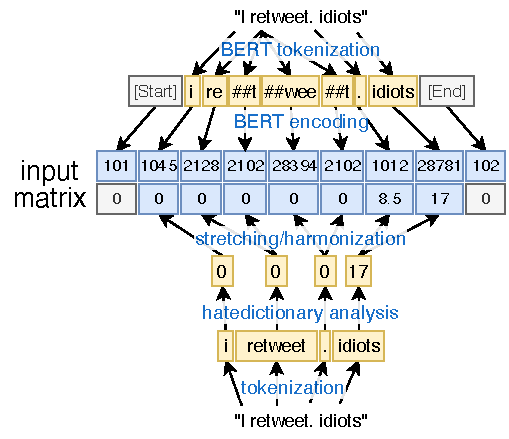
\includegraphics[width=5cm,keepaspectratio]{writing/02_final-report-latex/figures/processing-regular.pdf}
        \caption{Preprocessing of tweets and combination of BERT vectorisation with hate dictionary approach (own visualisation)}
        \label{fig:vectorization}
    \end{center}
\end{figure}

To harmonise the input for our CNN we pad the vector with zeros at the end until the vector has length $120$, as can be seen in Figure \ref{fig:padding1}.

\begin{figure}[ht]
    \begin{center}
        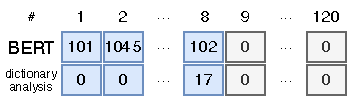
\includegraphics[width=5cm,keepaspectratio]{writing/02_final-report-latex/figures/processing-padding.pdf}
        \caption{Padding of the preprocessed tensor to harmonise the data set for the CNN (own visualisation)}
        \label{fig:padding1}
    \end{center}
\end{figure}

As discussed above, a convolution is used to combine multiple input values with different weights attached to them to an output value. We call the object that contains all the weights used in the calculation a kernel which is defined through the weight matrix $[w_{ij}]=W\in\mathbb{R}^{3 \times 3}$.

The first layer gets a 2D matrix $X\in\mathbb{R}^{2\times 120}$ of size length $120$ and height $2$ as input. Based on the settings for kernel size, stride, and dilation the kernel is applied to a sub-matrix $\tilde{X}$ of input matrix $X$.

We can define the application of the kernel to one sub-matrix mathematically as a function that takes the sub-matrix $\tilde{X}$ and a matrix of weights $W$ to calculate a weighted sum, i.e. the convolution:
$$f:\mathbb{R}^{3\times 3}\times\mathbb{R}^{3 \times 3}\rightarrow \mathbb{R}, \hspace{0.3cm}(\tilde{X},W)\mapsto \sum_{i,j=1}^3 w_{ij} x_{ij} =:y_* $$

The actual learning of the model is based on the weights that we train. A weight matrix is convoluted at every layer with sub-matrices of the input matrix to create a new output matrix. The matrix is padded again with zeros to ensure that the convolution with the matrix is not reducing the overall size of the matrix that is moving through the neural network. In Figure \ref{fig:convolution} a matrix with height $2$ is padded with one row of zeros to allow a kernel of size $3$ to reduce the matrix to an output of height $2$ again.

\begin{figure}[ht]
    \begin{center}
        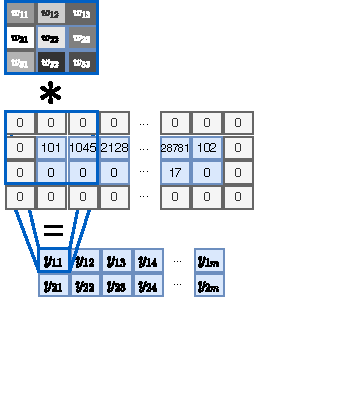
\includegraphics[width=5cm,keepaspectratio]{writing/02_final-report-latex/figures/processing-convolution.pdf}
        \caption{Convolution of weight matrix $W=[w_{ij}]$ with submatrix of padded input matrix to produce output matrix $Y=[y_{ij}]$ (own visualisation)}
        \label{fig:convolution}
    \end{center}
\end{figure}

Each neuron in our network comes with its own weight matrix. The initial weights for these weight matrices $W$ are generated randomly with a uniform distribution of values. All neurons in the first layer get the same input vector but will produce different convolutions due to the randomness of the weights.
If all weights would be equal then the back-propagation algorithm that tweaks the weights after each training step would have to change all of them or choose randomly which one to adjust because all would have the same effect. Randomisation of the weights takes this decision from the algorithm by "breaking symmetry" in the network \cite[p.~297]{Goodfellow-et-al-2016}. Thus, the randomisation is the precondition for the network to learn.

PyTorch calculates the range of values from which it can draw randomly from the amount of input values and the kernel size.
The possible weights must be in the range $(-\sqrt{k},+\sqrt{k})$, where $k:=\frac{1}{\text{input channels}\cdot\text{kernel size}}$.

If we look at all the convolutions happening in order to produce the output of one neuron, we can see that an individual input value is included in multiple weighted sums.
The choice of $k$ ensures that neurons with different kernel size and/or input channel amount produce convolutions that are in the same numerical range. This happens through a kind of normalisation in the definition of $k$.
Each neuron in the neural network has its own weights and draws them randomly from a uniform random distribution, e.g. $w_{11},w_{12},w_{21} \in\mathcal{U}(-\sqrt{k},\sqrt{k})$ like in Figure \ref{fig:initweights}.
\begin{figure}[ht]
    \begin{center}
        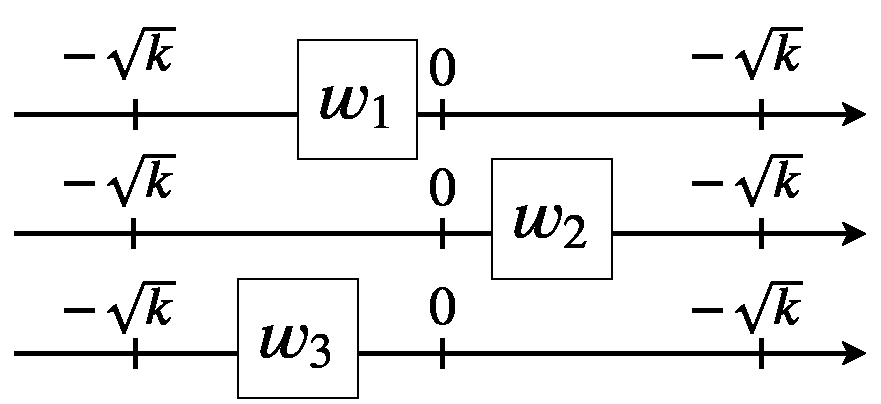
\includegraphics[width=5cm,keepaspectratio]{writing/01_midterm-report-latex/figures/intialization.pdf}
        \caption{Random initialisation of kernel weights (own visualisation)}
        \label{fig:initweights}
    \end{center}
\end{figure}


In each neuron the convolution is repeated for all sub-matrices of the vector (or only a part of it depending on kernel size, stride and dilation). This results in multiple matrix multiplication per neuron which applies the kernel to each sub-vector and outputs one matrix with thee result of all the associated convolutions (see Figure \ref{fig:convolution}).

Finally a bias $B$ is added to the convolution. The initial bias $B$ is drawn randomly from the same uniform distribution $\mathcal{U}(-\sqrt{k},\sqrt{k})$.

While the weights $W$ determine the focus of the calculations, the bias $B$ directly influences the result of the activation function of the neuron. If the activation function is a Sigmoid function (see Figure \ref{fig:sigmoid}) then e.g. a simple shift to the left (negative $b$) could reduce the whole neuron output to zero and thus make the information covered in the convolutions irrelevant for the network. The bias puts some neurons' activation threshold lower and some higher in the beginning, and allows the network to focus on the relevant information. As was mentioned above in relation to the weights, the initial randomisation of the bias allows the network to learn.
%
\begin{figure}[ht]
    \begin{center}
        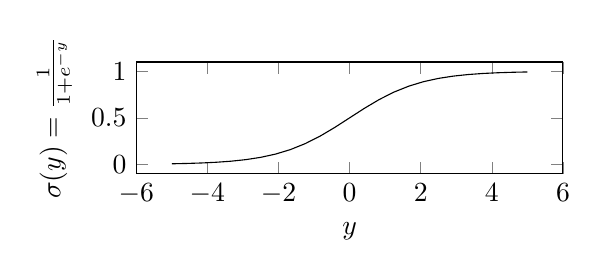
\begin{tikzpicture}
          \begin{axis}[
            height=3cm,
            width=7cm,
            ymax=1.1,
            ymin=-0.1,
            xlabel=$y$,
            ylabel={$\sigma(y) = \frac{1}{1+e^{-y}}$}
          ] 
            \addplot[mark=none] {1/(1+e^(-x))};
          \end{axis}
        \end{tikzpicture}
        \caption{Sigmoid function (own visualisation)}
        \label{fig:sigmoid}
    \end{center}
\end{figure}

%
The weights and the bias are adjusted depending on the loss after each training step through the back-propagation algorithm.


\end{document}